\chapter{Testing and Discussion of the Results}
\label{resultanddiscussion}

The nodes of the system are highly interconnected, therefore it is hard to test the nodes separately and with out influence on each other. This chapter includes the test setup for various nodes, as well as the test results and their discussion. Some of the test results introduce necessary optimizations to the system, which will be covered too. These optimizations will be tested by repeating the original test and comparing the results.

\section{Odometry Test}

The odometry is a key component in the navigation concept, since it will be used by multiple nodes and is the representation of the robots position in its environment.\\

Especially differential robots tend to have rotational error, when using the wheel-encoders to generate the odometry, since the wheels are forced to slip when the robot is turning.\\

To test the quality of the odometry the robot will be placed in the world pictured in Figure \ref{simworld}. Now the robot is supposed to drive one round, during which the odometry of the robot will be tracked.\\

In theory the trace of the odometry should be closed perfectly, after the robot performed its first round.\\

\subsection{Results}

When looking at the odometry published by the differential drive plugin during the test in Figure \ref{wheel odom} it is noticeable, that the measurement has a huge rotational error, which is expected, since the robot has a differential steering type.
The quality of the odometry obviously is not sufficient and has to be improved.
\begin{figure} 
	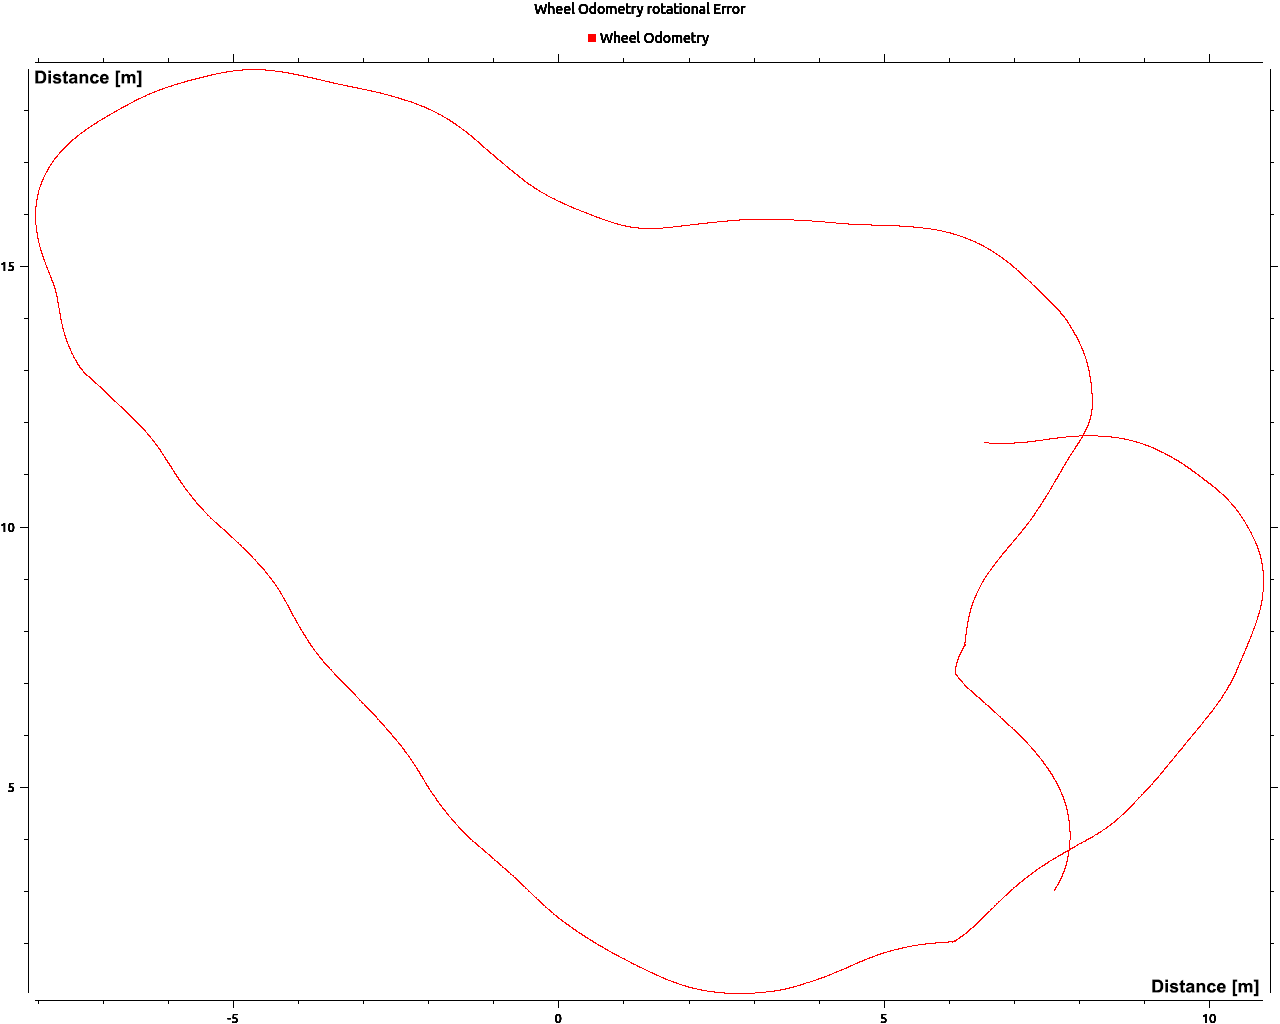
\includegraphics[width=\textwidth]{Pictures/rot error}
	\caption{Odometry test result}
	\label{wheel odom}

\end{figure}


\subsection{Optimization}
Since the odometry is found to not being sufficient for the navigation the following optimization approach will be tried and further testing will be performed. The test scenario will remain the same.

To improve the odometry the ROS package robot\_localization can be used. It provides an extended kalman filter for the fusion of sensor data for odometry.\\

To reduce the rotational error, an IMU (Inertia measurement unit) will be added to the robot configuration. Both, the IMU and the wheel encoder will be fused by robot\_localization.

The IMU provides the following data:
\begin{itemize}
	\item Orientation
	\item Angular velocity
	\item Linear acceleration
\end{itemize}

In this use case the IMU is only supposed to measure data relevant for 2D operation roll, pitch and translation in z (axis according to to REP 103) will not be passed to the filter. 

The IMU is used for localization purposes, therefore the linear acceleration data is not interesting, since the accelerations would need to be integrated twice to be used for the pose. This would amplify every little error in the measured acceleration and will decrease the reliability of the odometry with increasing time.\\

Accordingly the only things fused from the IMU are the yaw orientation and velocity.\\

Just like the IMU data the integration of the wheel-odometry data has to be discussed which consist only from linear and angular velocities, as well as a pose derived from the velocities.\\

Here the most interesting part is the y velocity since the robot is relying on differential drive steering and therefore not able to have instantaneous y acceleration other than drift.\\

In contrast to the acceleration values of the IMU the y velocity will be included since according to Tom Moore (the developer of robot\_localization) it will give certainty that the robot has not moved in the y direction\cite{robotlocalizationconfiguration}. Obviously the x and yaw velocity have to be included as well.

The position component of the wheel-odometry on the other hand will not be used, based on the fact that the position is already derived from the velocitys this would include the same data twice.\\

Unfortunately this does not solve the problem of the odometry correction yet. As visible in Figure \ref{pose comparison wheel odom + IMU} the odometry of the extended kalman filter has large jumps in it compared to the wheel-odometry. When observing it in real time the ekf odometry starts to drift and jumps back after a certain amount of time.\\
Looking at the linear velocities of both the ekf and the wheel odometry in Figure \ref{velocity comparison wheel odom + IMU} it is noticeable that the ekf filter does estimate a continuous acceleration, whereas the velocity of the wheel encoders actually decreases.\\



\begin{figure} 
	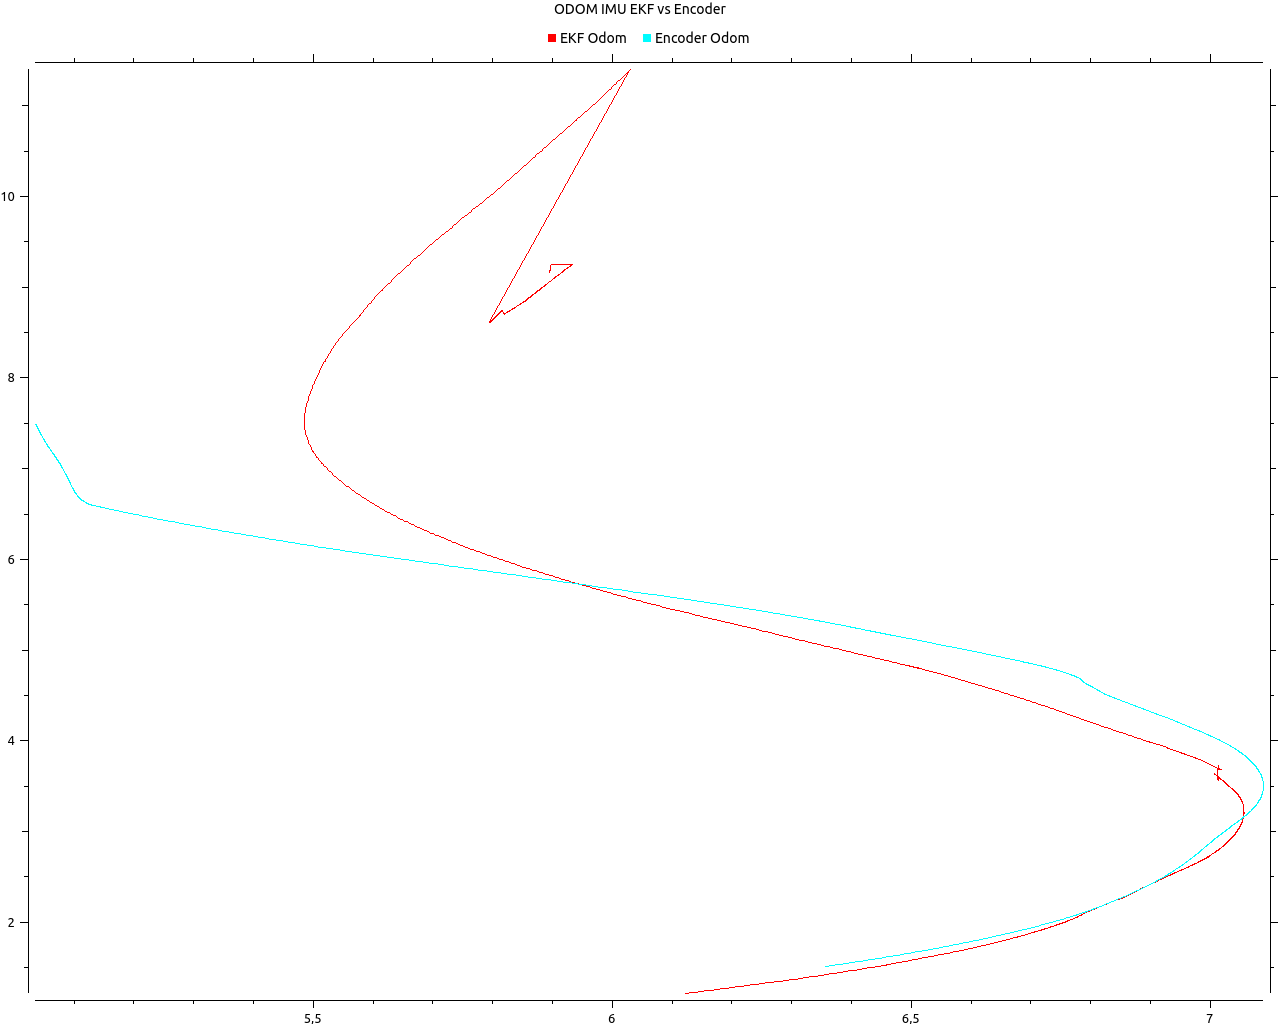
\includegraphics[width=\textwidth]{Pictures/odom pose comp}
	\caption{Pose comparison wheel odom + IMU}
	\label{pose comparison wheel odom + IMU}

\end{figure}

\begin{figure} 
	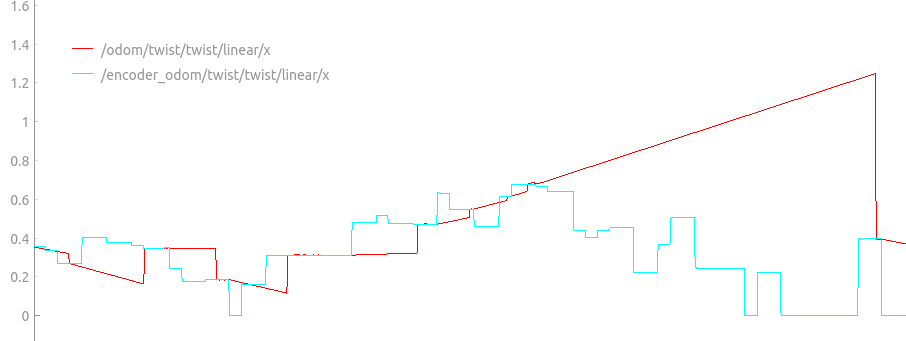
\includegraphics[width=\textwidth]{Pictures/comparison odom}
	\caption{Velocity comparison wheel odom + IMU}
	\label{velocity comparison wheel odom + IMU}

\end{figure}


To fix this, more data about the robots movement is required. Fortunately, robot\_localization has an input for command velocities such as velocities produced by move base. While the command velocity does not provide any measurement in the real world the ekf filter can profit from knowing what the velocity actually should be.\\

robot\_localization has a parameter for the timeout of the command velocity messages. Setting this lower than the cycle time of move\_base results in the offset pictured in figure \ref{velocity offset}. Therefore it is really important to configure this parameter to the current settings of move\_base.

\begin{figure} 
	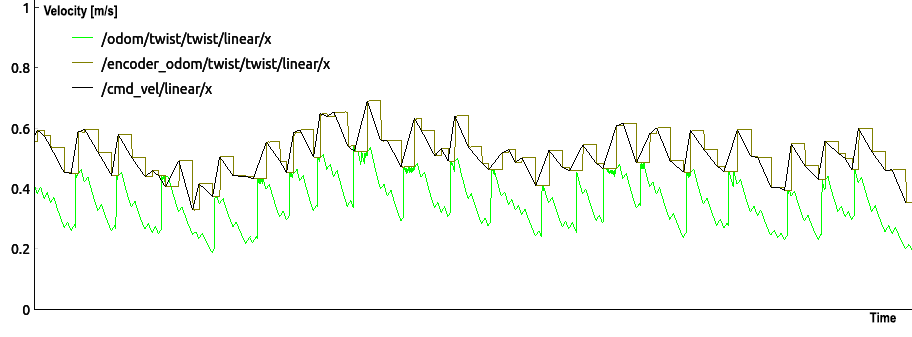
\includegraphics[width=\textwidth]{Pictures/velocity comp}
	\caption{Velocity offset caused by too low control timout}
	\label{velocity offset}

\end{figure}

After the inclusion of the command velocity, the acceleration limits in the configuration file of robot\_localization can be set equal to the limits in the local planner configuration.

When observing the results again it is noticeable, that the odometry has drastically improved as pictured in Figure \ref{Odometry comparison wheel odomIMUcmdvel}, equally the velocities stay closer together as pictured in \ref{velwithcmd}.

\begin{figure} 
	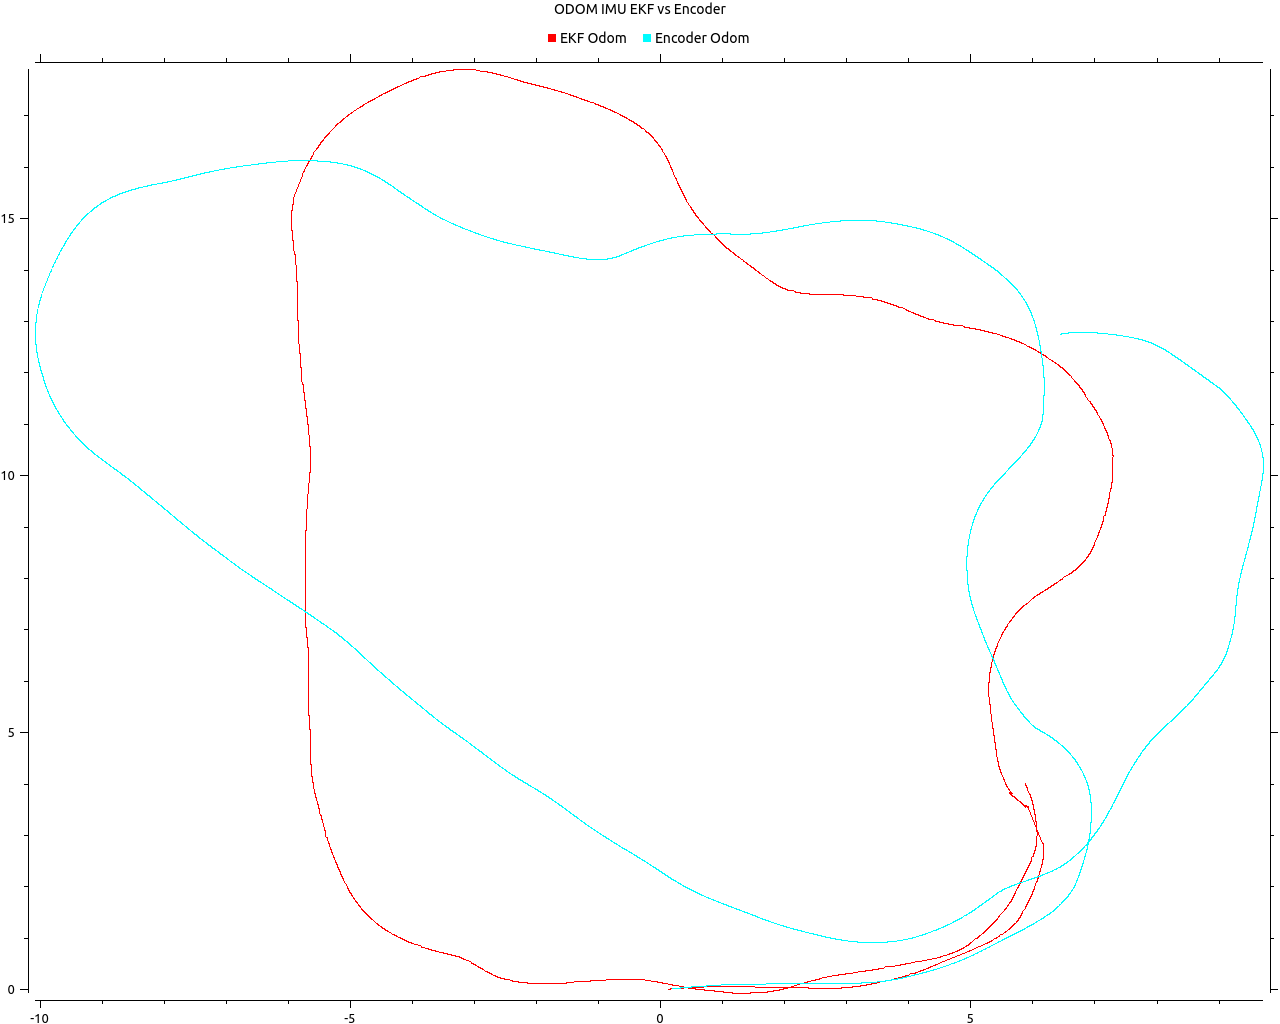
\includegraphics[width=\textwidth]{Pictures/odom after one round}
	\caption{Odometry comparison wheel odom + IMU + cmd\_vel}
	\label{Odometry comparison wheel odomIMUcmdvel}

\end{figure}
\begin{figure} 
	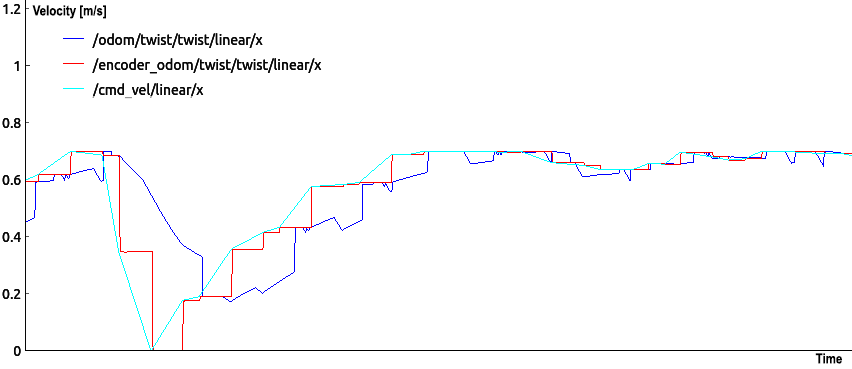
\includegraphics[width=\textwidth]{Pictures/circle vel}
	\caption{Velocity comparison with cmd\_vel}
	\label{velwithcmd}
\end{figure}



\begin{figure} 
	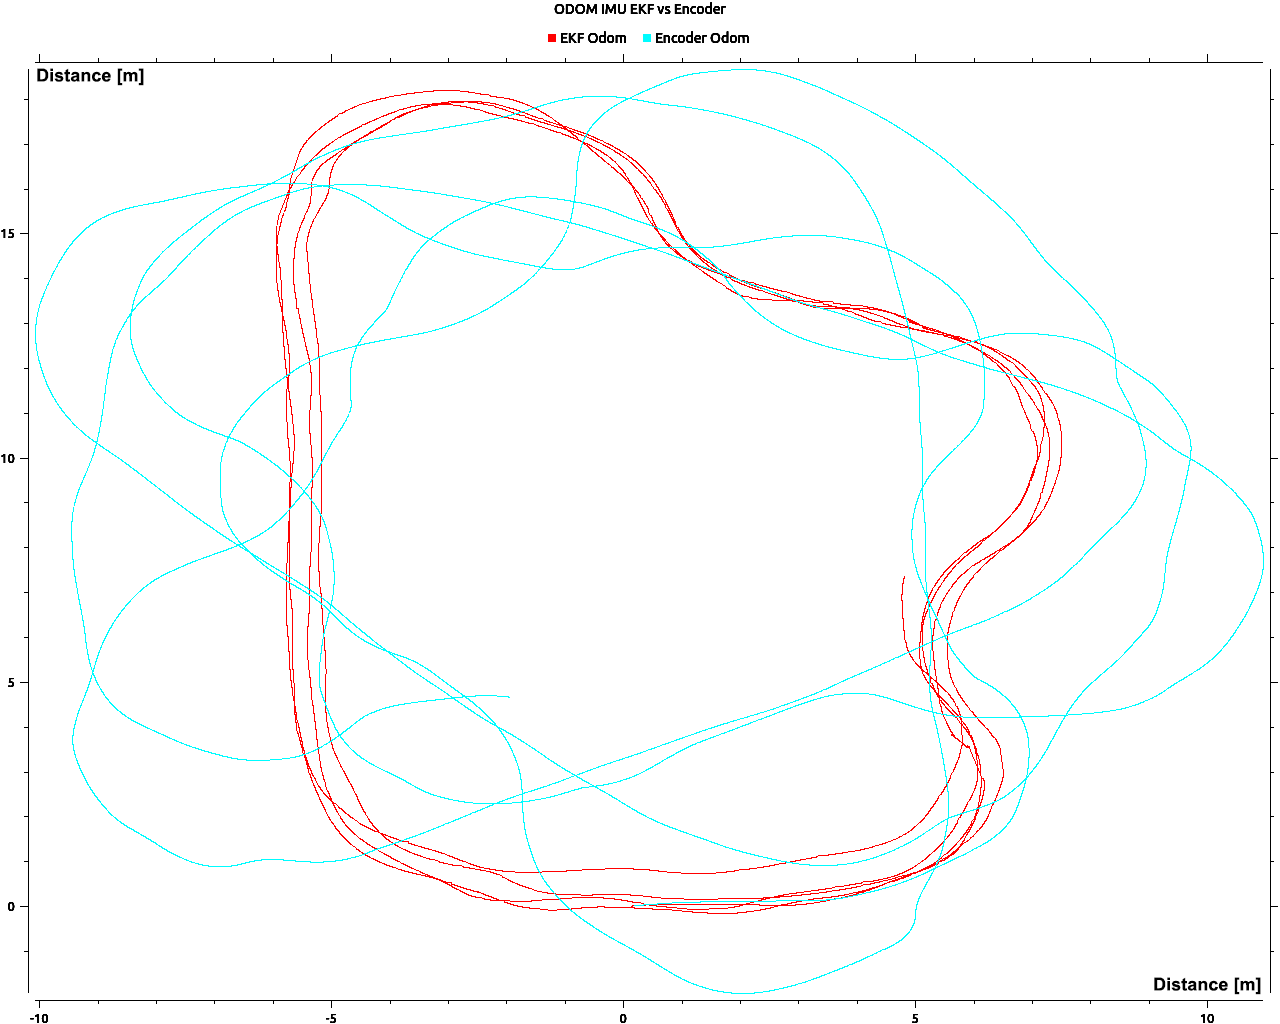
\includegraphics[width=\textwidth]{Pictures/odom comp multiple rounds}
	\caption{Odom comparison multiple rounds}
	\label{Odom comparison multiple rounds}

\end{figure}

Even after four rounds the odometry has not gained a large error in both translational and rotational as pictured in Figure \ref{Odom comparison multiple rounds}, furthermore the difference between the original odometry of the wheel encoders to the odometry from robot localization is quite remarkable.

After the rotational and translational errors are marginal the scale of the odometry needs to be checked.
To isolate the different errors from the scaling error a circular track is build with a radius of 10 meter. Since the turning radius is constant this isolates the rotational error which can be seen at the graph of the wheel odometry in Figure \ref{circular track}.\\
The radius was chosen that high so potential errors are amplified and easier detectable.\\
Since the robot is driving on the lane and not on the middle road marking the expected radius is 10,45 meter. When evaluating the EKF odom in Figure \ref{circular track} we see that the scale is very precise.
 
\begin{figure} 
	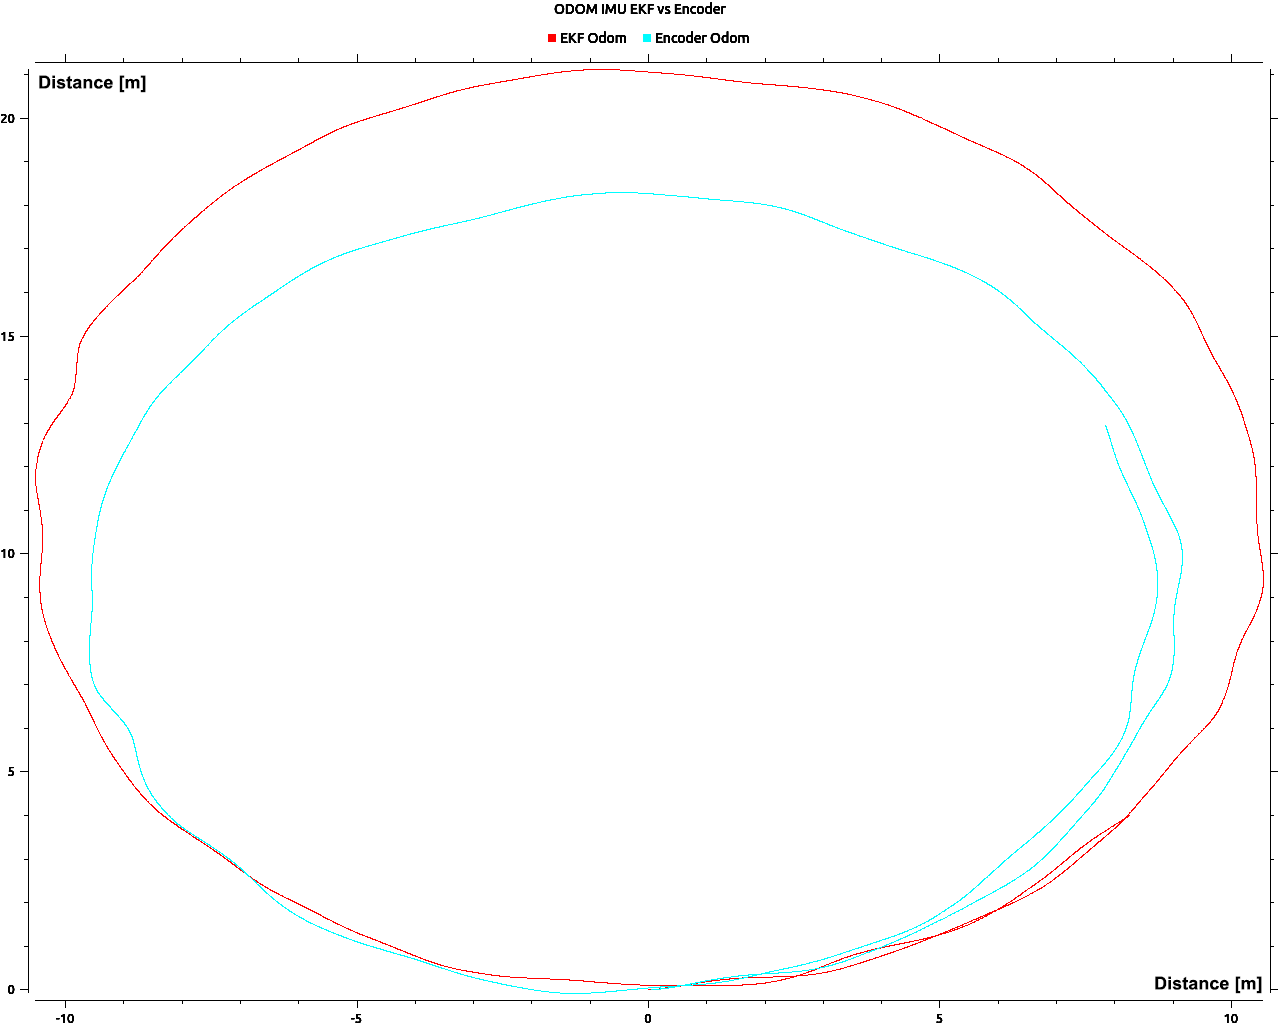
\includegraphics[width=\textwidth]{Pictures/circle odom}
	\caption{Odom comparison circular track}
	\label{circular track}

\end{figure}

As a final test the odometry from the robot\_localization node is compared to the true position from the simulation.

 \begin{figure} 
	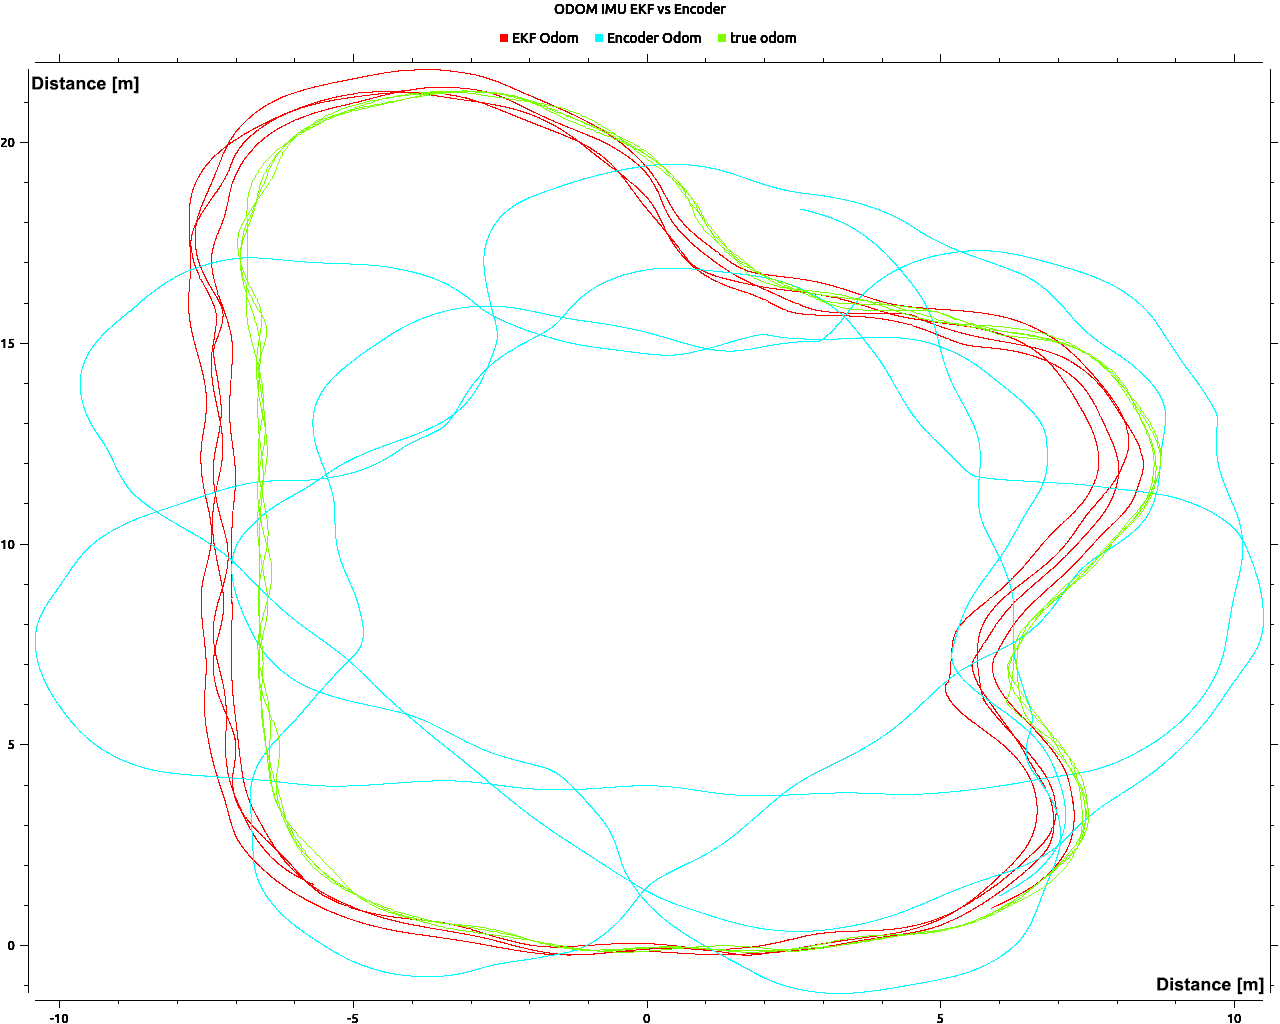
\includegraphics[width=\textwidth]{Pictures/odom with true}
	\caption{Comparison with true position}
	\label{trueodom}
\end{figure}

The comparison in Figure \ref{trueodom} shows, that the filtered odometry has a slight translational offset, but is very similar to the true odometry extracted from the simulation, hence it will be considered as sufficient for the navigation.\\
When comparing the pictured traces, with those pictured in \ref{Odom comparison multiple rounds} it is noticeable, that the oscillations of the red trace have increased. The setup of the test and the system in both tests are the same, which shows how difficult testing with the entire system is.

\section{Lidar Test}
The lidar is the only sensor, which detects static obstacles in the surrounding of the robot. Hence the quality of the data has to be checked.

To test the performance of the simulated lidar the robot will simply navigate in the world pictured in Figure \ref{simworld} and detect obstacles along the road.\\

The quality of the data will be observed by looking at the raw data, as well as the costmap, that receives the measurements of the lidar.\\

The evaluation of the costmap is necesarry, since it will mark measurements of the lidar as lethal. With increasing noise the marked obstacles will be less precise, therefore the lidar has direct influence on the performance of the navigation even when obstacles are not on the road.

The main focus of this test is sensor noise, since the Gazebo sensor plugin is configured based on the data sheet of the real lidar (Appendix \ref{AppendixDataSheets}).

\subsection{Results}
The lidar sensor is simulated with realistic noise and errors. This also introduces the well known edge error in laser distance measurement \cite{edgeeffect}. 

When using a ``realistic'' lidar to project obstacles into the costmap this error produces a lot of lethal point like obstacles that significately hinder navigation as visible in Figure \ref{unfiltered lidar}.

\begin{figure} 
	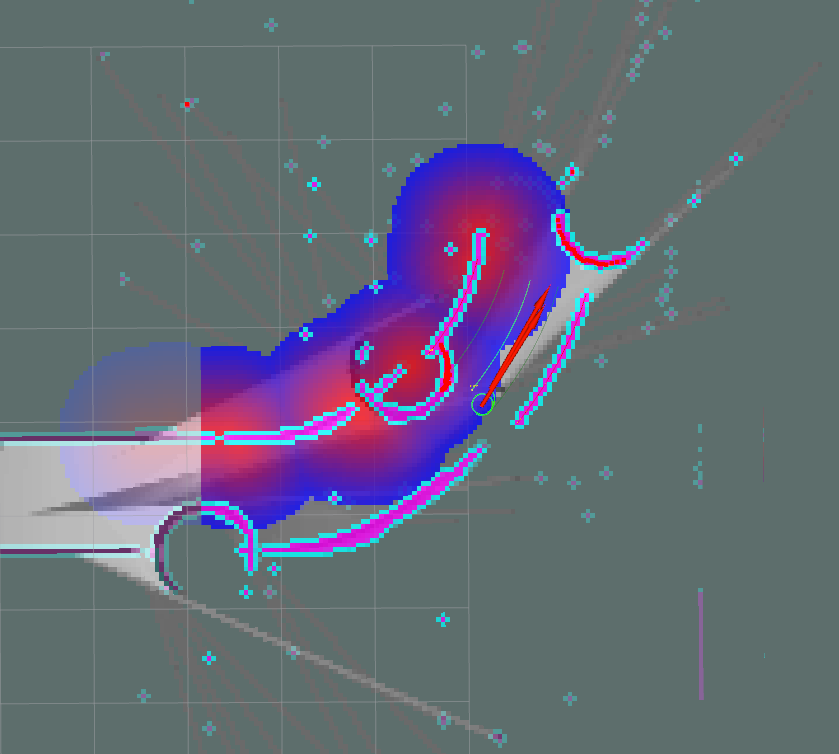
\includegraphics[width=\textwidth]{Pictures/Needs filtering of Laser}
	\caption{Lidar Test result}
	\label{unfiltered lidar}
\end{figure}

\subsection{Optimization}
To remove these error measurements the ROS package ``laser\_filters'' can be used. Among many different filter plugins it features the ``ScanShadowFilter'' that is developed to remove the veiling effect around obstacles cause by the edge effect \cite{laserfilters}.


Figure \ref{lasercomp} shows a comparison between the filtered and unfiltered laser scan, while keeping the data for 10 seconds. This allows to see the quickly jumping outliers caused by the edge effect. The filter seems well configured since the filtered points have no single outlier but still featuring a very good representation of the measured obstacle.

\begin{figure} [H]
	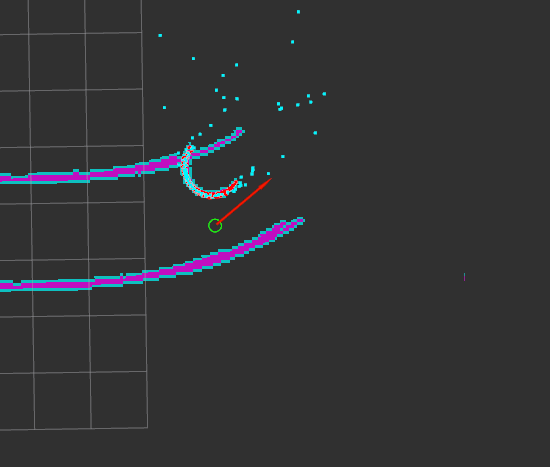
\includegraphics[width=\textwidth]{Pictures/LASERFILTER COMP}	
	\caption{Comparison between filtered and not filtered laser scan (red - filtered, turquoise - raw)}
	\label{lasercomp}
\end{figure}

\section{Road Detection Test}

As the road\_detection is the only data source providing informations about the road it is crucial for successful navigation.

To check if the road detection offers good enough results a long duration test will be performed, during which the output of the roadRecordEvaluation node will be monitored, which outputs the relation between the amount of recognized road and overall attempts to find a road.\\

The robot will navigate on the course pictured in Figure \ref{simworld} until the output of the roadRecordEvaluation settles to a reliable result.

\subsection{Results}
As pictured in figure \ref{longdurroad} the performance of the road detection converges to ca. 98.8\%. At the beginning the graph is not as reliable since there have not yet been enough measurements.\\

The duration of the test was roughly 1.5 hours of continuous navigation without obstacles in the simulation.

\begin{figure} 
	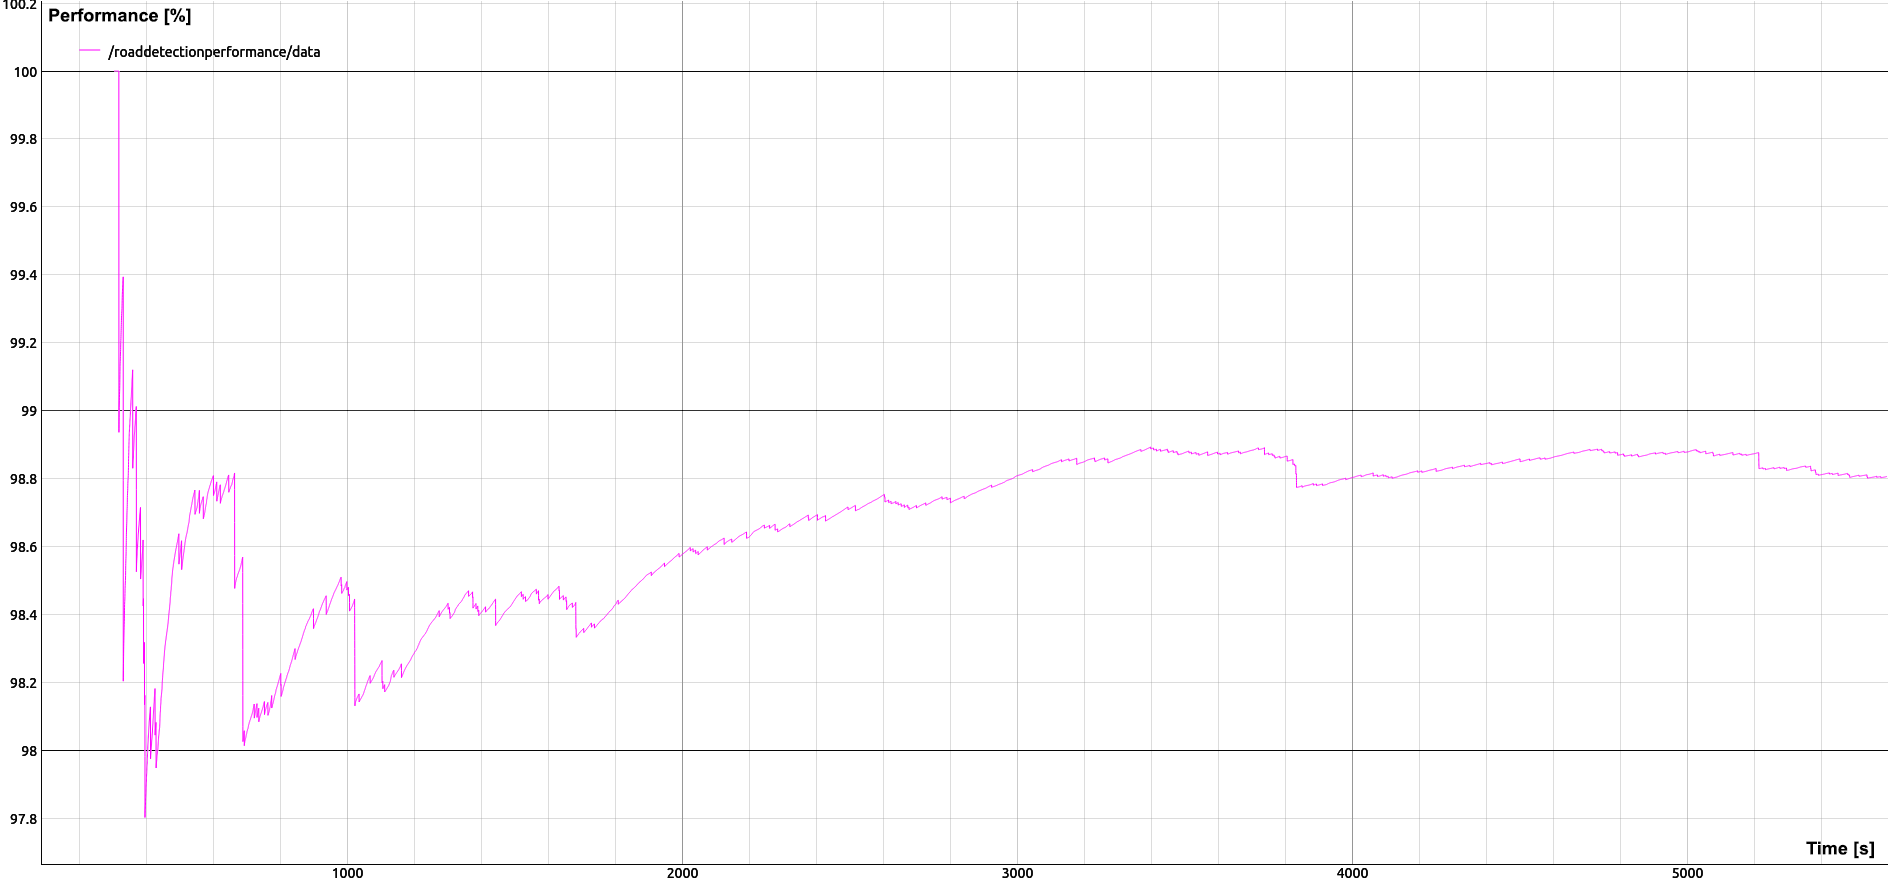
\includegraphics[width=\textwidth]{Pictures/long duration road detection test}
	\caption{RoadRecordEvaluation during long duration test}
	\label{longdurroad}
\end{figure}

\section{SLAM Test}
The SLAM algorithm chosen for the the concept is used in a very uncommon way, since it is not only receiving input from a real range finding sensor, but as well from the road detection.

The data from the road detection is very self similar, meaning that for example a straight section of road will always look very similar independent of its position like shown in figure \ref{selfsimilar}. The lack of details in the data from the road detection might complicate Cartographers scan matching.\\

\subsection{Test Scenarios}
The SLAM algorithm will be tested by limiting the data input and observing the resulting map. During this the navigation will solely work with the predicted goals, since it is yet unsure if the SLAM map is even usable. Cartographer will be tested in the following conditions:

\subsubsection{Data purely from road detection:}
The reason for this test is to check if the SLAM algorithm can handle mapping with as least information as possible. This will make loop-closure difficult and cartographer has to work with the self similar data only.\\
The aim is, that the robot can drive multiple rounds, on the track and cartographer produces an optimized map with little unmatched submaps and well connected road markings.\\

\subsubsection{Data purely from road detection and lidar scan with obstacles at the side of the road}
The used lidar (specified in Appendix \ref{AppendixDataSheets}) has a range of 4 m. Therefore it is likely, that the sensor sees obstacles that are next to the circuit of the Carolo-Cup, but are not on the track itself. These might be provide sufficient features for loop closure. Therefore the map could be very reliable after the first round. 
In this test the robot will be placed in the testing environment with obstacles next to the road as pictured in \ref{2slamtestenv}.

\begin{figure} 
\centering
	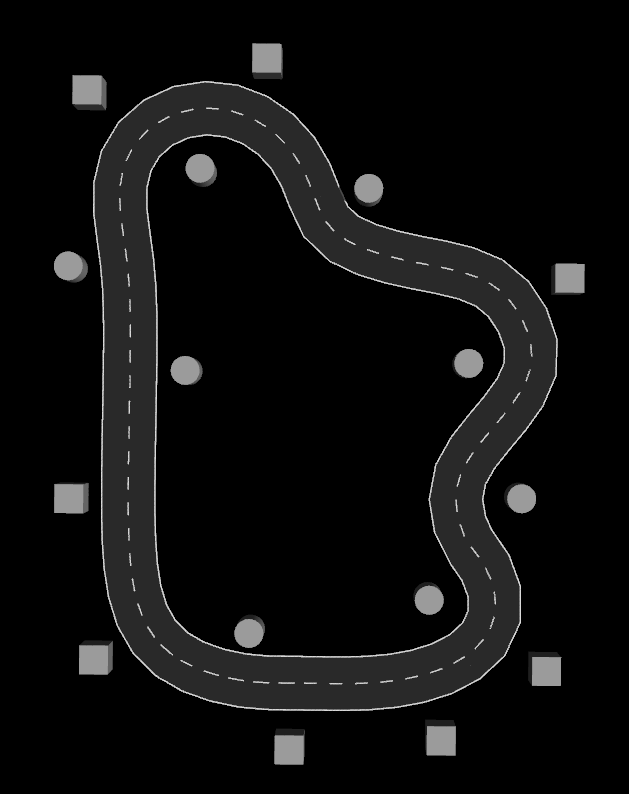
\includegraphics[width=.4\textwidth]{Pictures/2slamtest}
	\caption{Test environment with obstacles at the side of the road}
	\label{2slamtestenv}
\end{figure}

\subsubsection{Long duration test with both road detection and lidar scan with obstacles at the side of the road:}
Cartographer seems to not merge old submaps but process all of them always, which will progressively increase computational load. Since the SLAM is supposed to be used during mapping, this can become important with a lot of sensor inputs that offer constraint potential and long runtime.
The same setup as in the \nth{2} test will be used but the focus is on the moment, at which cartographer cannot optimize in real time caused by too many submaps and constraints.\\


\subsubsection{Data purely from localization and lidar scan with obstacles on the road:}
This test is meant to be the worst case for the SLAM algorithm during navigation. The purpose is to check how cartographer handles data loss during obstacle avoidance and lane swapping.
The obstacles will be placed in two corners and therefore in the edge case where the camera has the worst chance of seeing the road because of the steering angle, as well as on the straight section of the road to cover the case where the camera can not see the road during merging on an other lane. Furthermore the obstacles will be placed far enough apart so the lidar has only vision on one at the same time.\\

\subsection{Results}
\subsubsection{Data purely from road detection:}

The following pictures contain the SLAM map after the \nth{1},\nth{2} and \nth{3} round.\\

\begin{figure} 
	\centering
	\begin{subfigure}{.3\linewidth}
		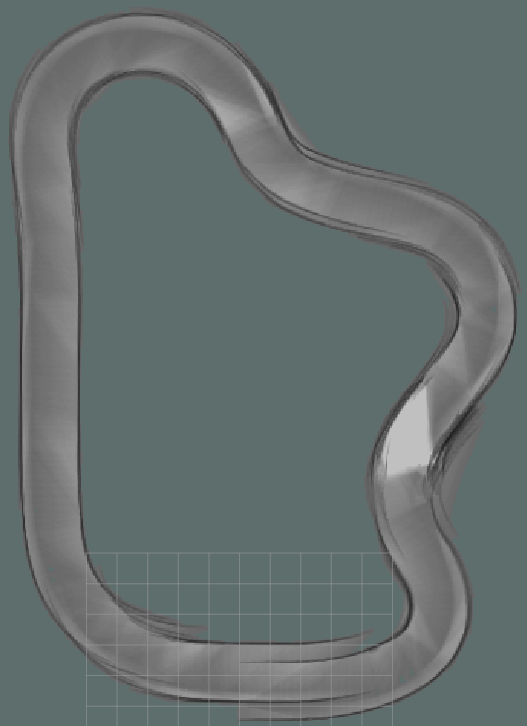
\includegraphics[width=\textwidth]{Pictures/1slamtest1}
		\caption{First}
		\end{subfigure}	
	%\hskip2em
	\begin{subfigure}{.3\linewidth}
		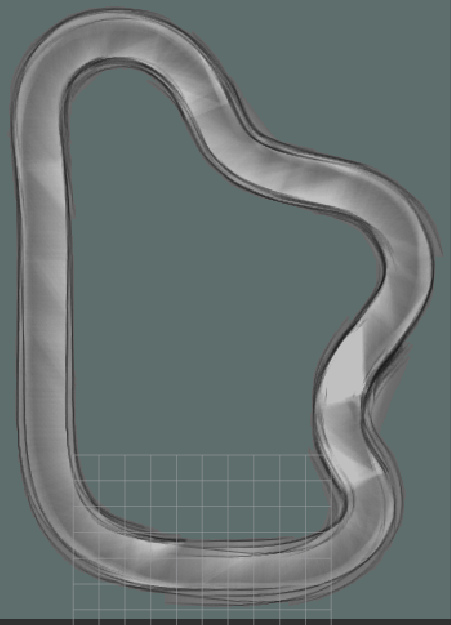
\includegraphics[width=\textwidth]{Pictures/1slamtest2}
		\caption{Second}
	\end{subfigure}
	%\hskip2em
	\begin{subfigure}{.3\linewidth}
		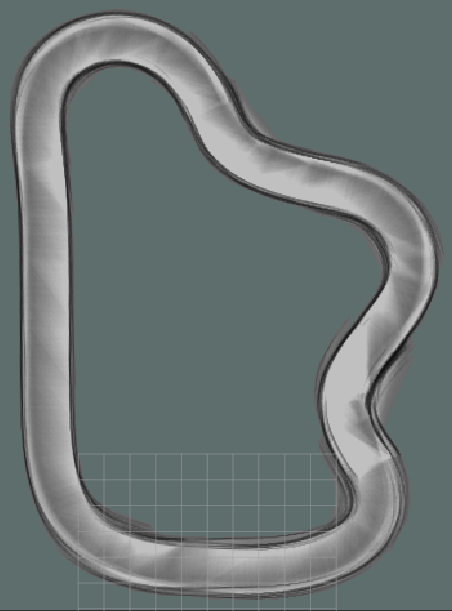
\includegraphics[width=\textwidth]{Pictures/1slamtest3}
		\caption{Third}
	\end{subfigure}

	\caption{SLAM map of first three rounds}
	\label{1slamtest}

\end{figure}

In the first round the map is not yet optimized. Like pictured in  figure \ref{1slamtest} the road is not connected at the bottom after the first round, but has slight translational error.\\
In the second round the road is closed, but some submaps are slightly misaligned which can be seen by the blurry road markings.\\
This is well corrected in the third round and will improve from here on with every round, until the computational effort is too high.\\

\textbf{Data purely from road detection and lidar scan with obstacles on the side of the road:}\\


As pictured in figure \ref{2slamtest} Cartographer manages to close the road already after the first round. After the second round the road borders are slightly blurry, therefore the submaps are not yet perfectly matched. This blurriness slightly improves after the third round, but the submaps are not yet perfectly matched with each other.

\begin{figure} 
	\centering
	\begin{subfigure}{.3\linewidth}
		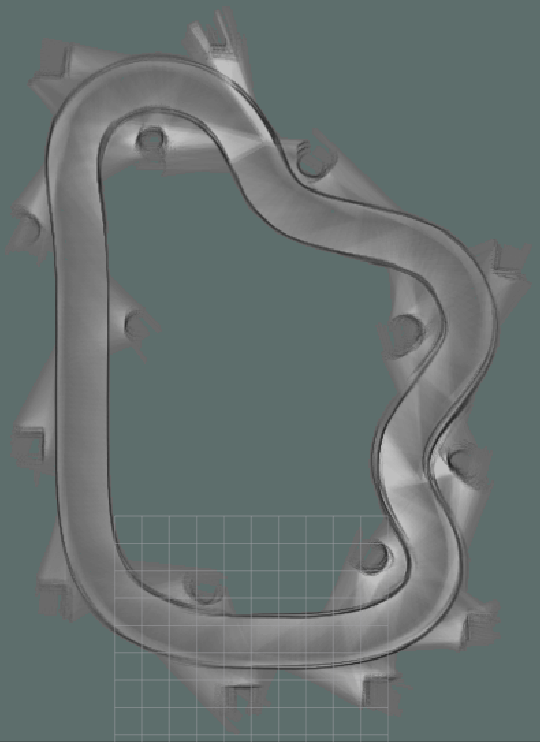
\includegraphics[width=\textwidth]{Pictures/2slamtest1}
		\caption{\nth{1} round}
		\end{subfigure}	
	%\hskip2em
	\begin{subfigure}{.3\linewidth}
		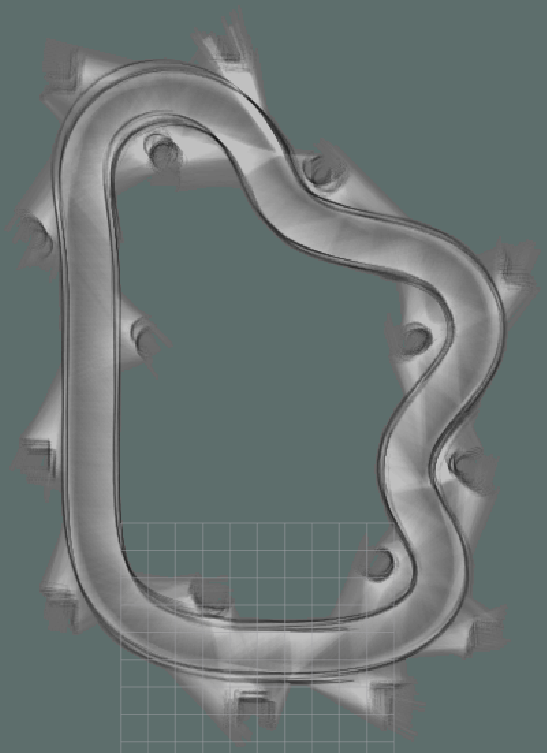
\includegraphics[width=\textwidth]{Pictures/2slamtest2}
		\caption{\nth{2} round}
	\end{subfigure}
	%\hskip2em
	\begin{subfigure}{.3\linewidth}
		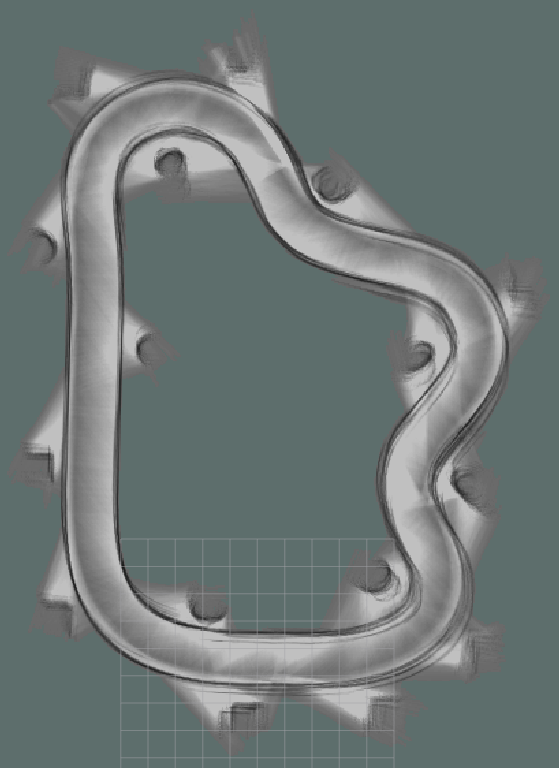
\includegraphics[width=\textwidth]{Pictures/2slamtest3}
		\caption{\nth{3} round}
	\end{subfigure}

	\caption{SLAM map of first three rounds}
	\label{2slamtest}

\end{figure}



\textbf{Long duration test with both road detection and lidar scan with obstacles on the side of the road:}\\

The map built by Cartographer during this test shows, that it is a very good representation of the real environment over the first four rounds as pictured in Figure \ref{3slamtest}.\\

After the \nth{7} round it is noticeable, that the matching of submaps seems to take more and more time, which is visible by a trace of unmatched submaps, that are slightly shifted. This is caused by the computational burden caused by the amount of submaps. In this round the Cartographer node already takes up 20\% of the cpu resources and increases continuously. At this point realtime scan and submap matching is not possible anymore, resulting in enormous processing delays.

\begin{figure} 
	\centering
	\begin{subfigure}{.3\linewidth}
		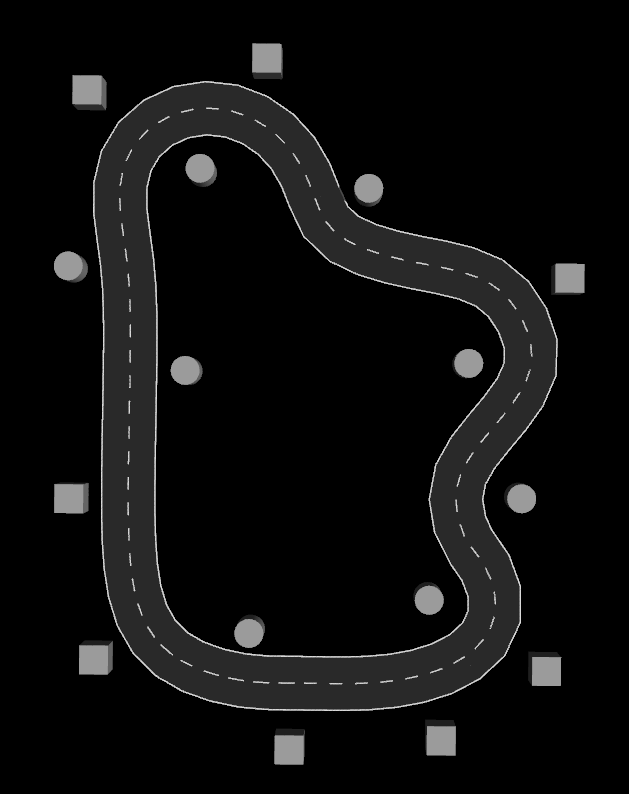
\includegraphics[width=\textwidth]{Pictures/2slamtest}
		\caption{Real Environment}
		\end{subfigure}	
	%\hskip2em
	\begin{subfigure}{.3\linewidth}
		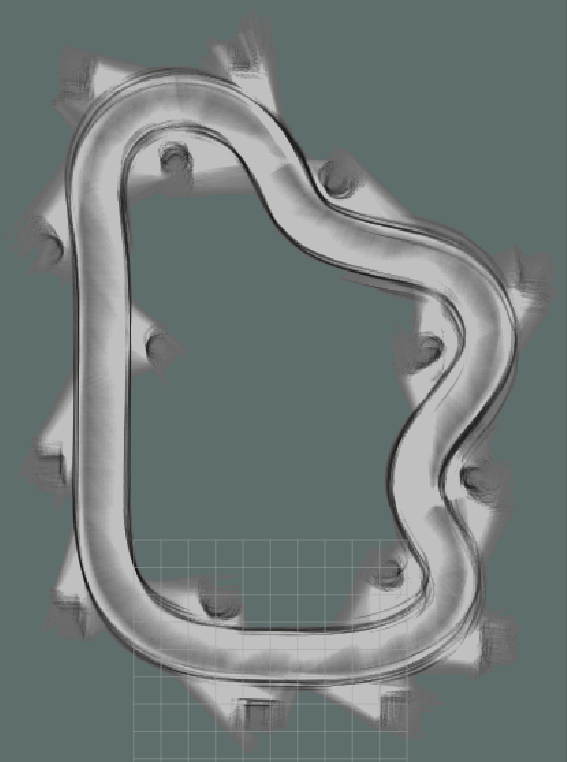
\includegraphics[width=\textwidth]{Pictures/2slamtest4}
		\caption{\nth{4} round}
	\end{subfigure}
	%\hskip2em
	\begin{subfigure}{.3\linewidth}
		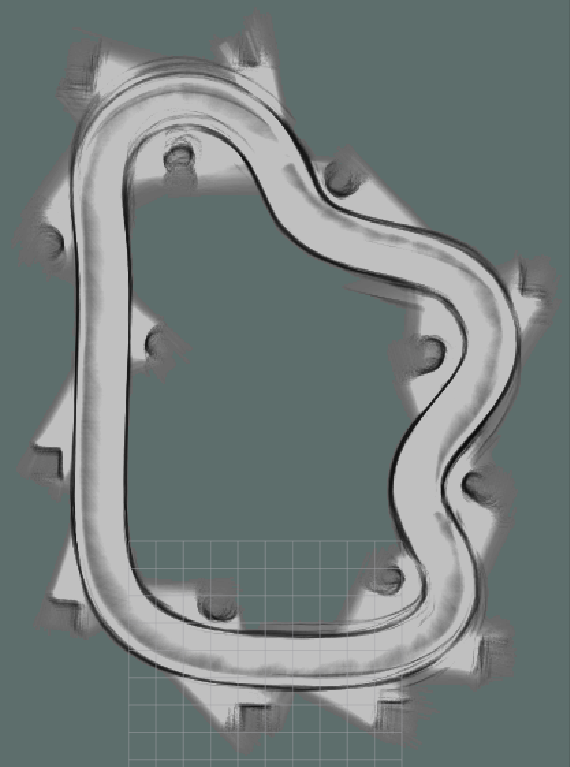
\includegraphics[width=\textwidth]{Pictures/2slamtest7}
		\caption{\nth{7} round}
	\end{subfigure}

	\caption{SLAM map rounds during long duration test}
	\label{3slamtest}

\end{figure}


\textbf{Data purely from localization and lidar scan with obstacles on the road:}\\

\begin{figure} 
	\centering
	\begin{subfigure}{.3\linewidth}
		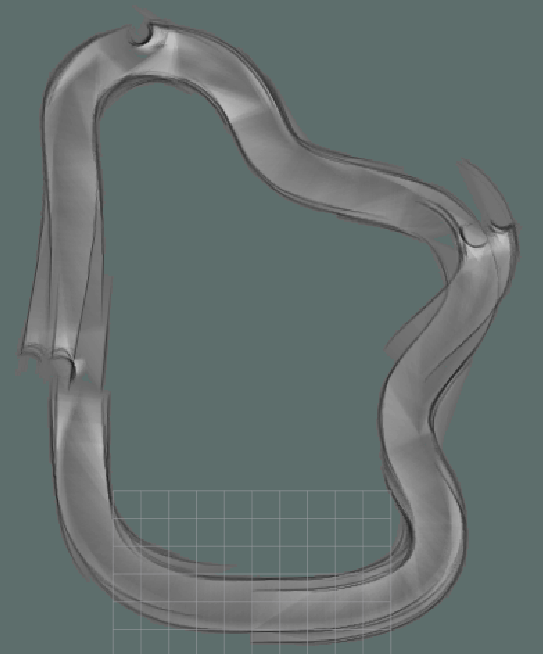
\includegraphics[width=\textwidth]{Pictures/3slamtest1}
		\caption{\nth{1} round}
		\end{subfigure}	
	%\hskip2em
	\begin{subfigure}{.3\linewidth}
		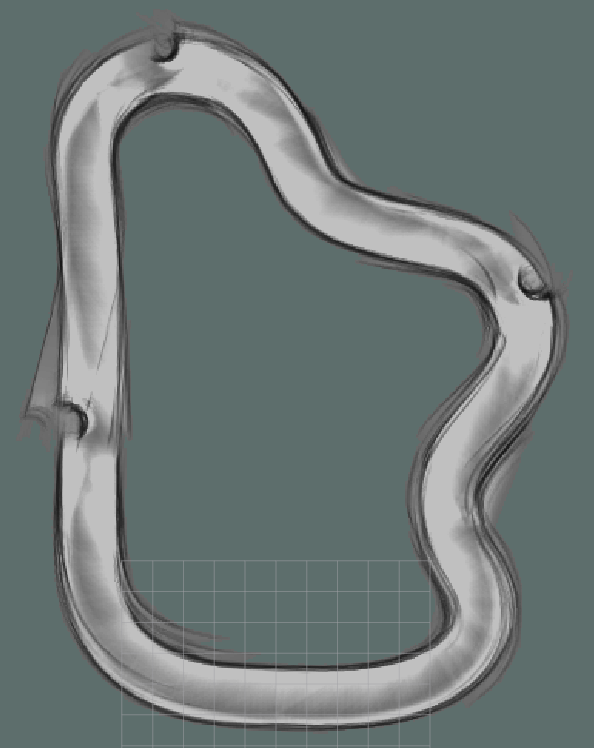
\includegraphics[width=\textwidth]{Pictures/3slamtest4}
		\caption{\nth{4} round}
	\end{subfigure}
	%\hskip2em
	\begin{subfigure}{.3\linewidth}
		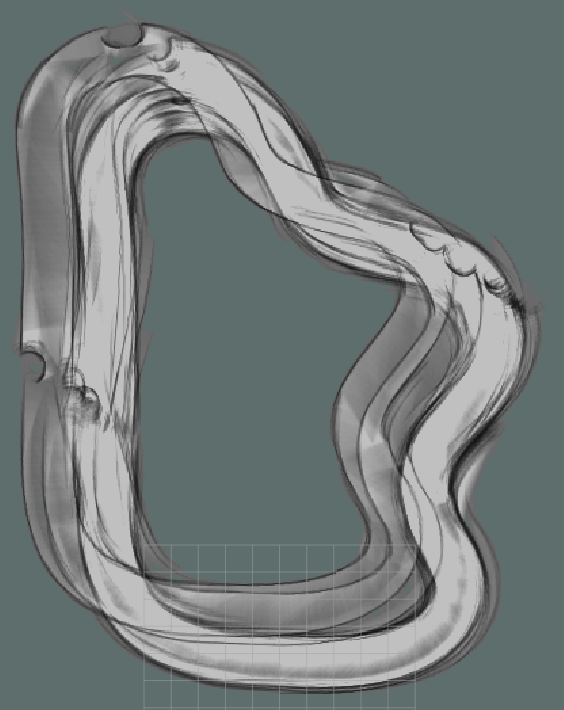
\includegraphics[width=\textwidth]{Pictures/3slamtest10}
		\caption{\nth{10} round}
	\end{subfigure}

	\caption{SLAM map rounds during long duration test}
	\label{4slamtest}

\end{figure}

As pictured in Figure \ref{4slamtest} Cartographer struggles with aligning the submaps during obstacle avoidance and suffers from rotational error.\\
Fortunately these errors are mostly corrected over the period of the next few rounds.\\ In the \nth{10} round however Cartographer suffers from the same issue highlighted by the long duration test. Here it is clearly visible, that the queue of unmatched submaps is more than one entire round.\\

\textbf{Discussion of the SLAM test results}\\
As proven by the first two tests, Cartographer is well tuned and the map would be useable for goal extraction. The submaps are well alligned and the map has no huge translational or rotational offset.\\

The \nth{3} and \nth{4} test on the other hand display the limitations of the slam algorithm in this use case.\\
When obstacles are located on the right lane the allignment of the submaps fails and a lot of submaps can't be attached to the rest of the map. After passing the same obstacle in multiple rounds the map improves to a point where it would be usable for goal extraction.\\
The \nth{3} test proves that Cartographer is not usable in SLAM mode during long time navigation an a circuit. This is caused by the amount of submaps that are close to each other and the resulting amount of constraints between each of them.\\

Based on these test results it is not feasible to use the SLAM map for navigation with obstacles on the road, since the map is just not reliable enough.




\section{Complete System Test}

After the previous tests the entire concept has to be tested in order to check, if the concept in its entirety works as anticipated.

Autonomous navigation in the following test scenarios will be performed:

\begin{itemize}
	\item no obstacles
	\item obstacles on left lane
	\item obstacles on right lane
\end{itemize}

During all test the following criteria will be monitored as well as any unexpected problems during the test:

\begin{itemize}
	\item distance to the right lane when no obstacle is close
	\item obstacle avoidance distance to object
\end{itemize}

For these tests the exact position of the obstacles and the robot will be used for evaluation. This allows to determine the exact distance between the robot and obstacles, as well as if the robot is still on the road.\\
The distance to the right lane will be determined by using the polynomial provided by the road detection. A so called ``avoidance'' starts when the robot is just slightly over the middle line, without any hysteresis.

As defined in the rules of the Carolo-Cup the merging onto the right lane during the obstacle avoidance is supposed to take place within the next two meters after an obstacle \cite{carolocup}.

In all tests the robot will drive multiple rounds if possible to produce reliable results. The tests will be performed in the environment pictured in Figure \ref{simworld}.\\

\subsection{Results}
The following subsections cover the discussion of the complete system tests.\\\\
\textbf{No obstacles}\\
The reason for this test is, to check how good the robot stays on the right lane. Therefore, the robot drives in the described test environment, while the difference between the right lane and the robot center is monitored.

\begin{figure} 
	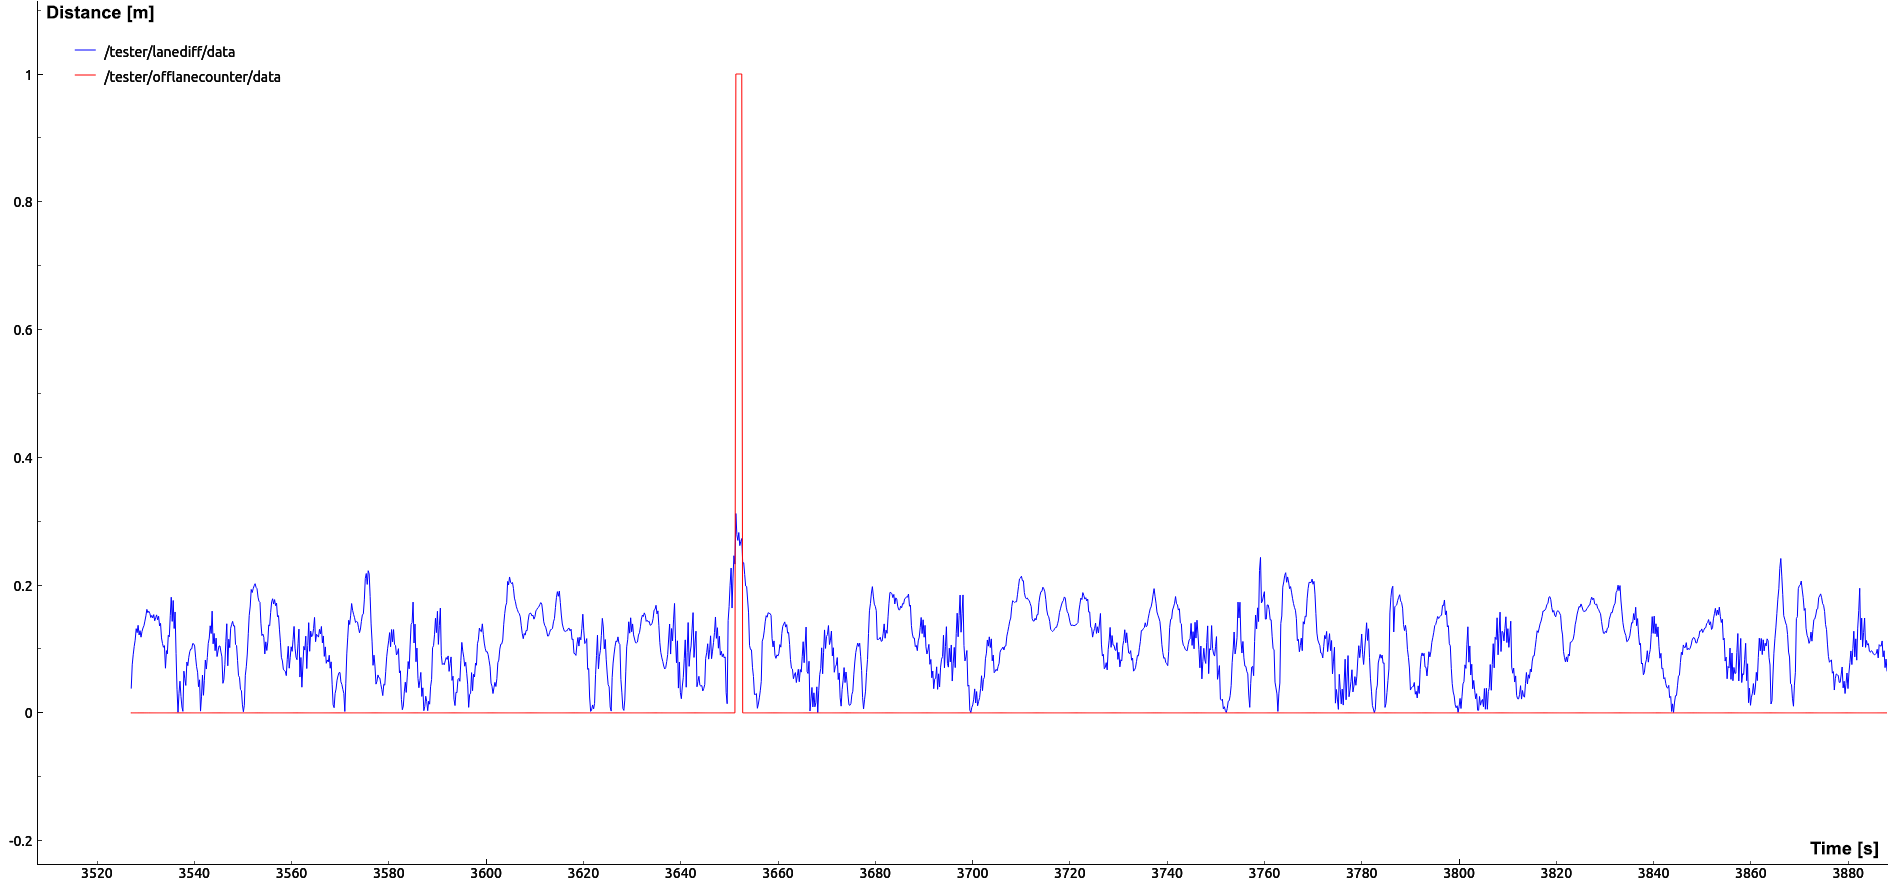
\includegraphics[width=\textwidth]{Pictures/final analysis no obstacle}
	\caption{Absolute error of the robot trajectory and rectified signal of the avoidance duration}
	\label{noobserr}
\end{figure}

As pictured in Figure \ref{noobserr} the robot has left the road markings once, caused by the bug of the global planner described in Section \ref{globalplannertest}. During all other rounds the robot stayed on the right lane while having slight oscillations.\\
\begin{figure} 
	\begin{subfigure}{.5\linewidth}
		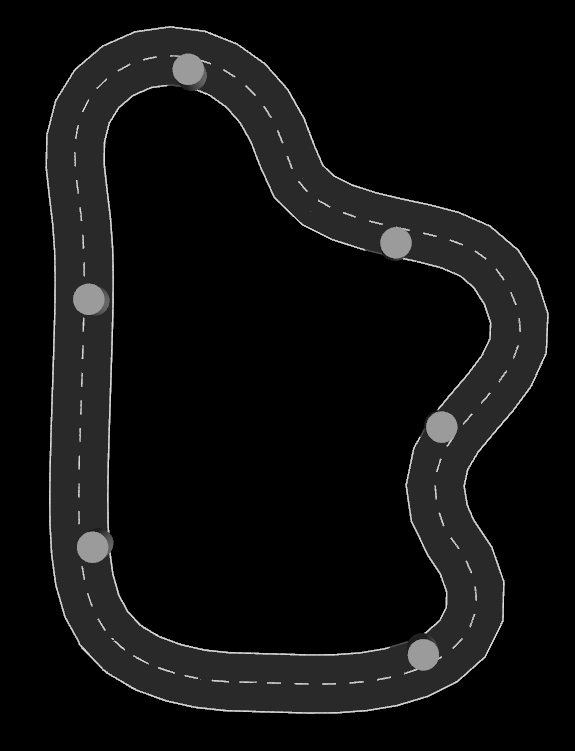
\includegraphics[width=\textwidth]{Pictures/obstacle left final 2}
		\caption{Obstacles on left lane}
	\end{subfigure}	
	%\hskip2em
	\begin{subfigure}{.5\linewidth}
		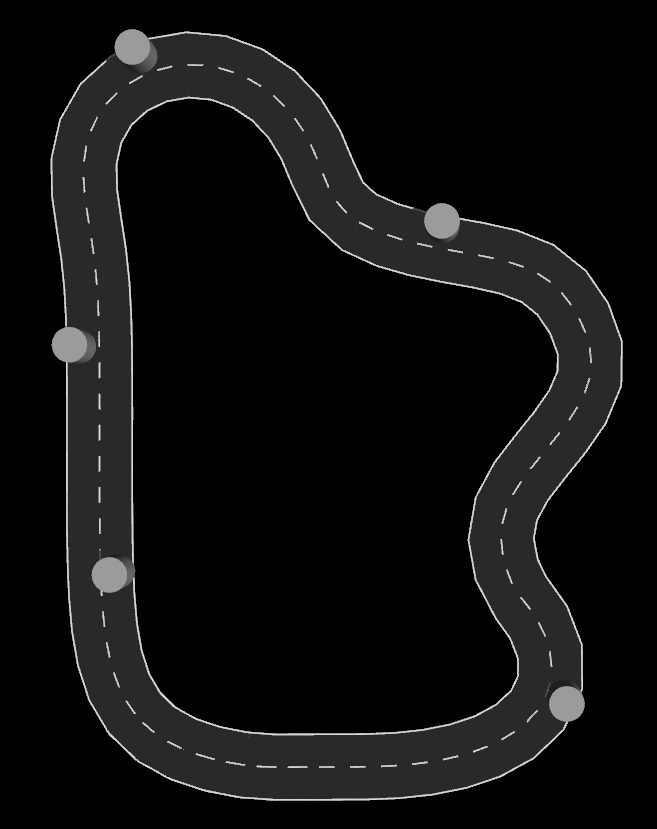
\includegraphics[width=\textwidth]{Pictures/right final obs}
		\caption{Obstacles on right lane}
	\end{subfigure}

	\caption{Obstacle placement for both final tests}
	\label{obstaclefinaltest}

\end{figure}
\textbf{Obstacles on left lane}\\
This test is supposed to test the behavior of the navigation when obstacles block the view of the camera but the robot has to drive on the right side as pictured in \ref{obstaclefinaltest} (a). In this test the robot will not drive as many rounds, since the goal is to observe the behavior when passing goals. In contrast to figure \ref{noobserr} the distance to the nearest obstacle will be included in the graph, thus it can be determined, if the robot left the lane because it is near an obstacle or not, for this the true positions from the simulation will be used. The obstacle distance will only be tracked, if it is below 3 meters.
\begin{figure} 
	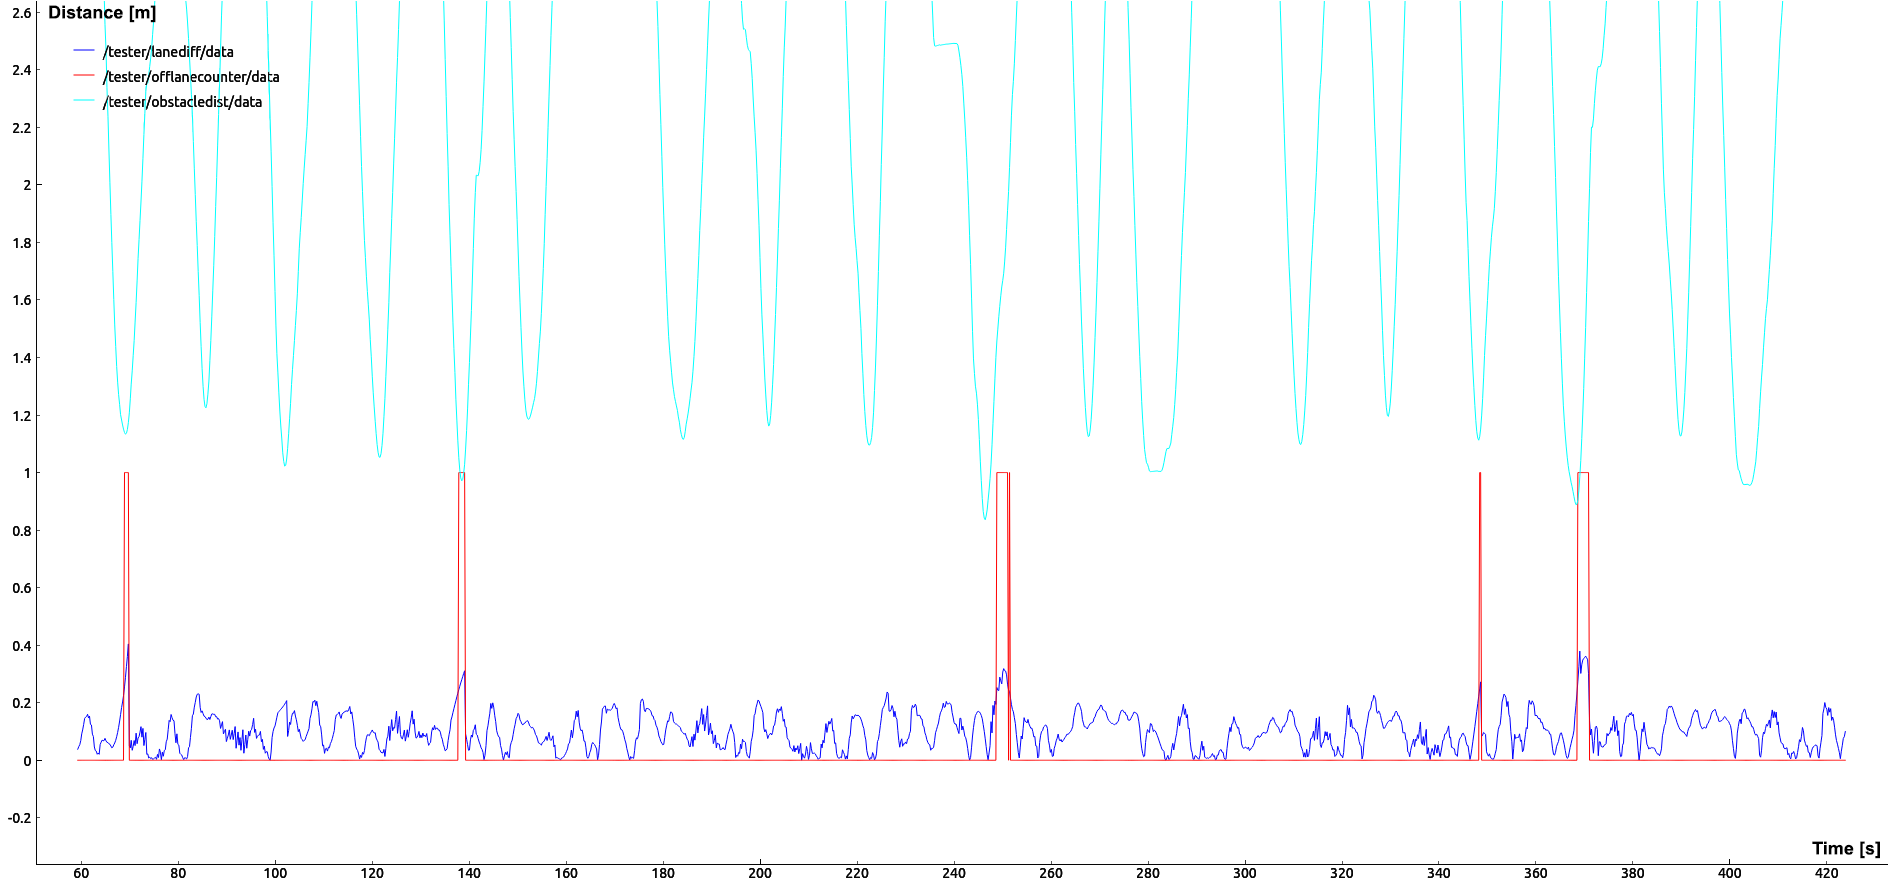
\includegraphics[width=\textwidth]{Pictures/left obs final obs2}
	\caption{Graph of left lane obstacle test}
	\label{leftobsfinal}
\end{figure}
As visible in figure \ref{leftobsfinal} the robot left the right lane way more often compared to Figure \ref{noobserr}. This suggests, that the robot is leaving the right lane, right after passing an obstacle. At this moment, the costmap does not yet contain any data about the road, since the road detection does not detect the road, after getting close to the obstacle. Therfore, the navigation drives starts to drive a straight line towards the goal, leading to the robot driving off the right lane.\\

\textbf{Obstacles on right lane}\\

To cover the possible scenarios of the Carolo-Cup this test is supposed to be a realistic application with a few obstacle scattered over the entire environment on the right lane like pirctured in \ref{obstaclefinaltest} (b). Like in the last test the obstacles will be located as well in corners, as on straight sections of the road.

\begin{figure} 
	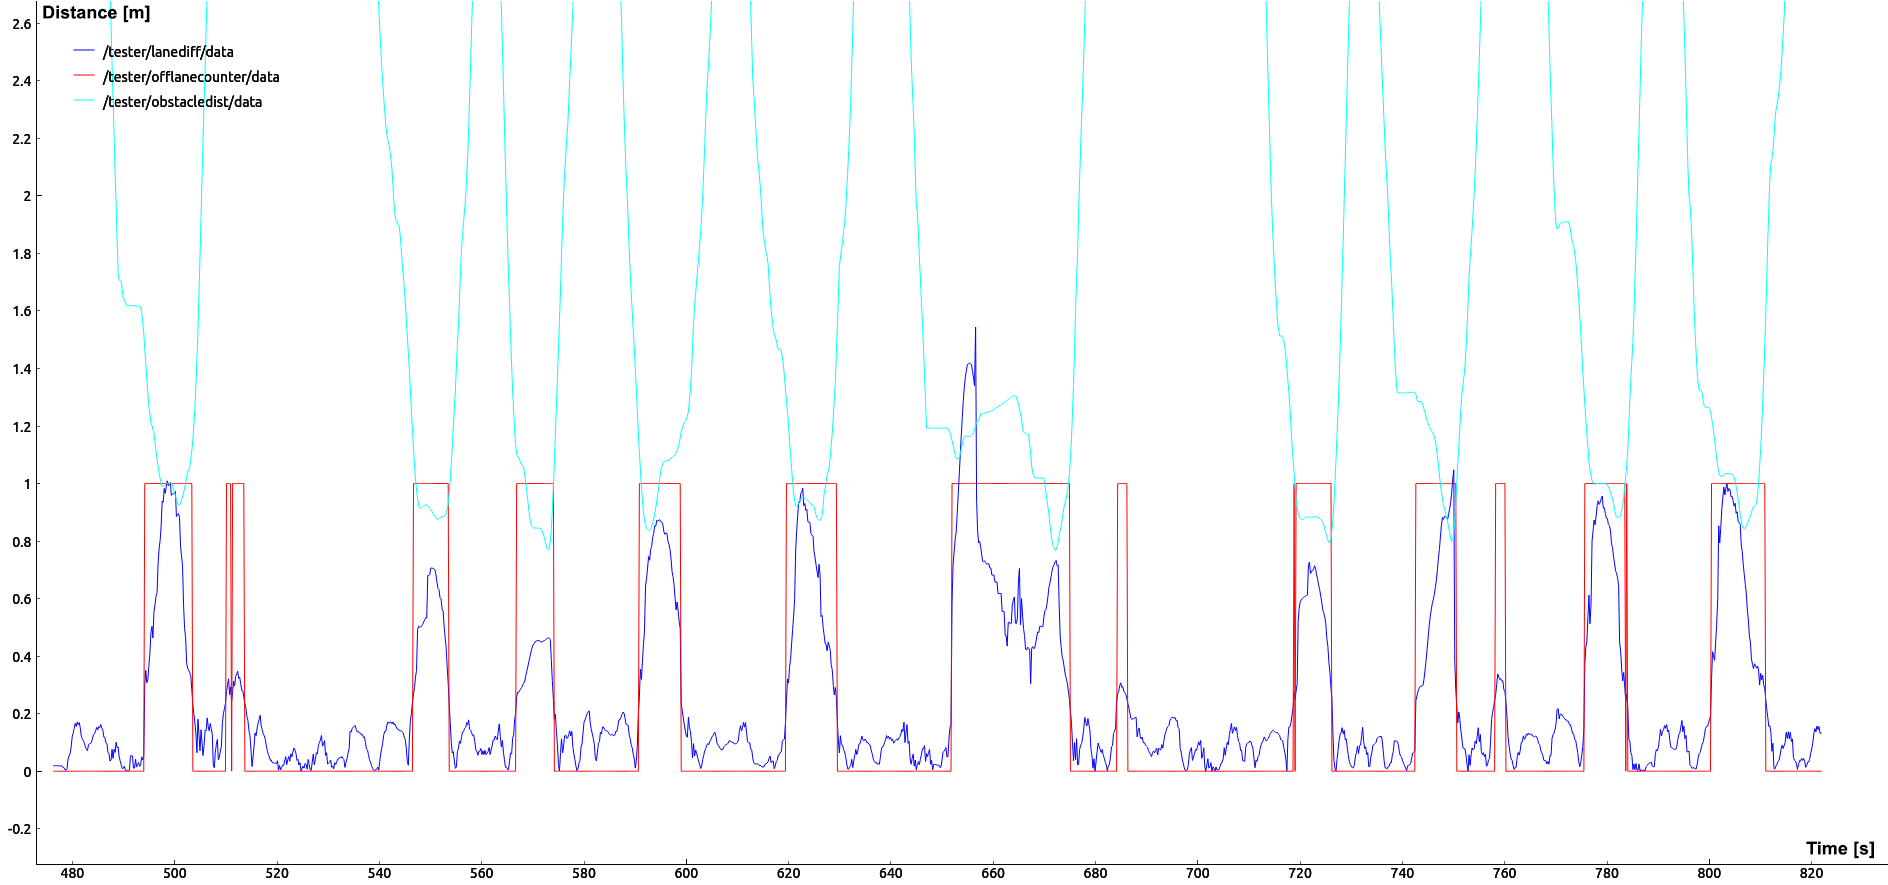
\includegraphics[width=\textwidth]{Pictures/right obs final obs}
	\caption{Graph of right lane obstacle test}
	\label{rightobsfinal}
\end{figure}


As pictured in Figure \ref{obstaclefinaltest} (b), there are five obstacles on the right lane. These can be seen, when inspecting the graph in Figure \ref{rightobsfinal}, which shows two rounds of the robot.

Furthermore the graph shows, that the robot successfully avoided all obstacles in both rounds. Unfortunately the robot left the right lane three times, when no obstacle in the proximity of it.\\

In the middle of the graph the robot took particularly long for the avoidance.

The graph also shows, that the avoidance is always finished before the robot is two meters away from the obstacle and therefore satisfies this condition.

\subsection{Discussion}

The results of the complete system tests show, that the navigation performs really well during simple lane following, since the road detection recognizes the road almost always as shown in the road\_detection test.

While observing the robot when it drives past obstacles on the left lane it was noticeable, that the robot mostly left the lane directly after it passed an obstacle in or directly after a corner.\\ 
In this case the predicted goal pulls the robot into the middle of the road since the costmap does not have information about the road and therefore will not force the global plan to the right lane. The approximated goal is still constructed with the circle approximation since the upcoming straight section has not been seen, which places the goal next to the lanes but not certainly on the right one.\\

Obstacle avoidance suffers from a similar problem. As shown in the ``Obstacle on the right lane'' test. Here it is visible, that the robot passes the obstacle nicely, but afterwards drives along the center of the road, which causes the spikes of the rectified signal visible in Figure \ref{rightobsfinal} after the avoidance. As soon as the robot has passed an obstacle fully, it drives straight to the latest predicted goal while waiting on new data from the road detection. Only, when the road detection supplies new information about the environment, the navigation is able to generate a plan to the right lane.



